\documentclass{standalone}

\usepackage[latin1]{inputenc}
\usepackage{amsmath}
\usepackage{amssymb}
\usepackage{amsthm}

\usepackage{tikz}
\usetikzlibrary{arrows}

%% generates a tightly fitting border around the work
%\usepackage[active,tightpage]{preview}
%\PreviewEnvironment{tikzpicture}
%\setlength\PreviewBorder{0.5mm}
%%\renewcommand\PreviewBbAdjust{-\PreviewBorder 1mm -1.15mm -0.85mm}

\usepackage{color}

%\pagestyle{empty}

\begin{document}

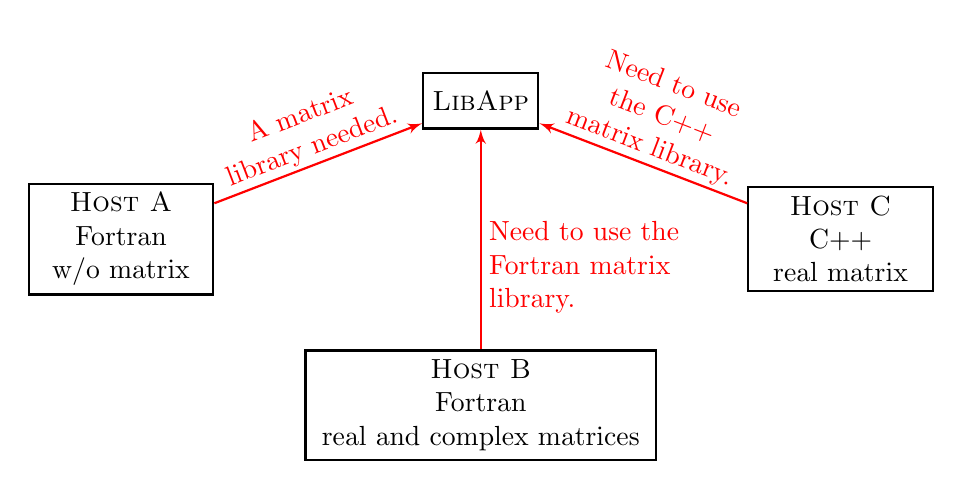
\begin{tikzpicture}[thick, node distance=50]
  \node[color=black, rectangle, draw, text badly centered, sharp corners, %
        minimum height=20] (LibApp) {\textsc{LibApp}};
  \node[color=black, rectangle, draw, text badly centered, sharp corners, %
        minimum height=20, text width=60, below of=LibApp, xshift=-130] (HostA) %
       {\textsc{Host A}\\Fortran\\w/o matrix};
  \node[color=black, rectangle, draw, text badly centered, sharp corners, %
        minimum height=20, text width=120, below of=LibApp, yshift=-60] (HostB) %
       {\textsc{Host B}\\Fortran\\real and complex matrices};
  \node[color=black, rectangle, draw, text badly centered, sharp corners, %
        minimum height=20, text width=60, below of=LibApp, xshift=130] (HostC) %
       {\textsc{Host C}\\C++\\real matrix};
  \draw [color=red, -latex'] (HostA) %
    edge node[align=center, midway, rotate=21, yshift=12, text width=70] %
    {A matrix library needed.}(LibApp);
  \draw [color=red, -latex'] (HostB) %
    edge node[align=left, midway, xshift=38, yshift=-10, text width=70] %
    {Need to use the Fortran matrix library.}(LibApp);
  \draw [color=red, -latex'] (HostC) %
    edge node[align=center, midway, rotate=-21, yshift=18, text width=70] %
    {Need to use the C++ matrix library.}(LibApp);
\end{tikzpicture}

\end{document}
